\documentclass[12pt]{article}
\usepackage{amsmath}
\usepackage{graphicx} % Required for including images
\usepackage[utf8]{inputenc}
\usepackage[style=apa, backend=biber, sorting=nyt]{biblatex}
\addbibresource{references.bib}

\title{Step-by-Step Linear Regression Fitting and Gradient Descent Optimization}
\author{Mike Sasso}
\date{September 28, 2024}

\begin{document}

\maketitle

\newpage

\section*{Data Points}
\[
(x, y) = \{(1, 4), (-2, 3), (3, 6), (4.5, 8), (0, 2), (-4, -3), (-1, -2), (4, 7), (-1, 2.5)\}
\]

\section*{Mean Calculation}
\[
\bar{x} = \frac{1 + (-2) + 3 + 4.5 + 0 + (-4) + (-1) + 4 + (-1)}{9} = \frac{4.5}{9} = 0.5
\]
\[
\bar{y} = \frac{4 + 3 + 6 + 8 + 2 + (-3) + (-2) + 7 + 2.5}{9} = \frac{27.5}{9} \approx 3.06
\]

\section*{Linear Regression Hypothesis}
The linear regression hypothesis function is:
\[
h_\theta(x) = \theta_0 + \theta_1 x
\]
Where: \\
- \( \theta_0 \) is the intercept. \\
- \( \theta_1 \) is the slope.

\section*{Cost Function \( J(\theta_0, \theta_1) \)}
To optimize the regression model, we minimize the cost function \( J(\theta_0, \theta_1) \), which measures the difference between the predicted and actual values:
\[
J(\theta_0, \theta_1) = \frac{1}{2m} \sum_{i=1}^{m} \left( h_\theta(x^{(i)}) - y^{(i)} \right)^2
\]
Where: \\
- \( m \) is the number of data points. \\
- \( h_\theta(x^{(i)}) = \theta_0 + \theta_1 x^{(i)} \) is the predicted value for each \( x^{(i)} \).\vspace{0.5cm}
\\
The errors are squared in the cost function to ensure that both positive and negative errors are treated equally, and larger errors are penalized more heavily.

\section*{Optimization via Gradient Descent}
To minimize the cost function, we use the gradient descent algorithm, which iteratively updates \( \theta_0 \) and \( \theta_1 \) to move toward the values that minimize the cost function. At each step, we calculate the gradient (the partial derivatives) of the cost function with respect to \( \theta_0 \) and \( \theta_1 \) and update them in the opposite direction of the gradient.

The update rules are:
\[
\theta_0 := \theta_0 - \alpha \frac{\partial}{\partial \theta_0} J(\theta_0, \theta_1)
\]
\[
\theta_1 := \theta_1 - \alpha \frac{\partial}{\partial \theta_1} J(\theta_0, \theta_1)
\]
Where: \\
- \( \alpha \) is the learning rate, a hyperparameter that controls the size of the steps taken in the gradient descent process. A larger \( \alpha \) results in bigger steps, while a smaller \( \alpha \) leads to smaller steps. \\
- \( \frac{\partial}{\partial \theta_0} J(\theta_0, \theta_1) \) and \( \frac{\partial}{\partial \theta_1} J(\theta_0, \theta_1) \) are the partial derivatives of the cost function with respect to \( \theta_0 \) and \( \theta_1 \), respectively, which tell us how much the cost function changes with respect to each parameter. \vspace{0.5cm}
\\

The gradient descent process continues until the change in \( \theta_0 \) and \( \theta_1 \) between iterations is smaller than a threshold, indicating that we have found the optimal values.


\section*{Partial Derivatives of the Cost Function}
The partial derivatives of the cost function with respect to \( \theta_0 \) and \( \theta_1 \) are:
\[
\frac{\partial}{\partial \theta_0} J(\theta_0, \theta_1) = \frac{1}{m} \sum_{i=1}^{m} \left( h_\theta(x^{(i)}) - y^{(i)} \right)
\]
\[
\frac{\partial}{\partial \theta_1} J(\theta_0, \theta_1) = \frac{1}{m} \sum_{i=1}^{m} \left( \left( h_\theta(x^{(i)}) - y^{(i)} \right) \cdot x^{(i)} \right)
\]
Using these partial derivatives, we update \( \theta_0 \) and \( \theta_1 \) incrementally in the direction that decreases the cost function until the algorithm converges on the optimal values.

\section*{Slope Calculation (\(\theta_1\))}
Now, applying the least squares method, the slope is calculated as:
\[
\theta_1 = \frac{\sum_{i=1}^{n} (x_i - \bar{x})(y_i - \bar{y})}{\sum_{i=1}^{n} (x_i - \bar{x})^2}
\]
\[
\theta_1 = \frac{77.75}{66} \approx 1.178
\]

\section*{Intercept Calculation (\(\theta_0\))}
The intercept is calculated using the formula:
\[
\theta_0 = \bar{y} - \theta_1 \bar{x}
\]
\[
\theta_0 = 3.06 - 1.178 \times 0.5 = 2.471
\]

\section*{Final Linear Regression Equation}
The final regression model equation is:
\[
y = \theta_0 + \theta_1 x = 2.471 + 1.178x
\]
\newpage
\begin{figure}[h]
    \centering
    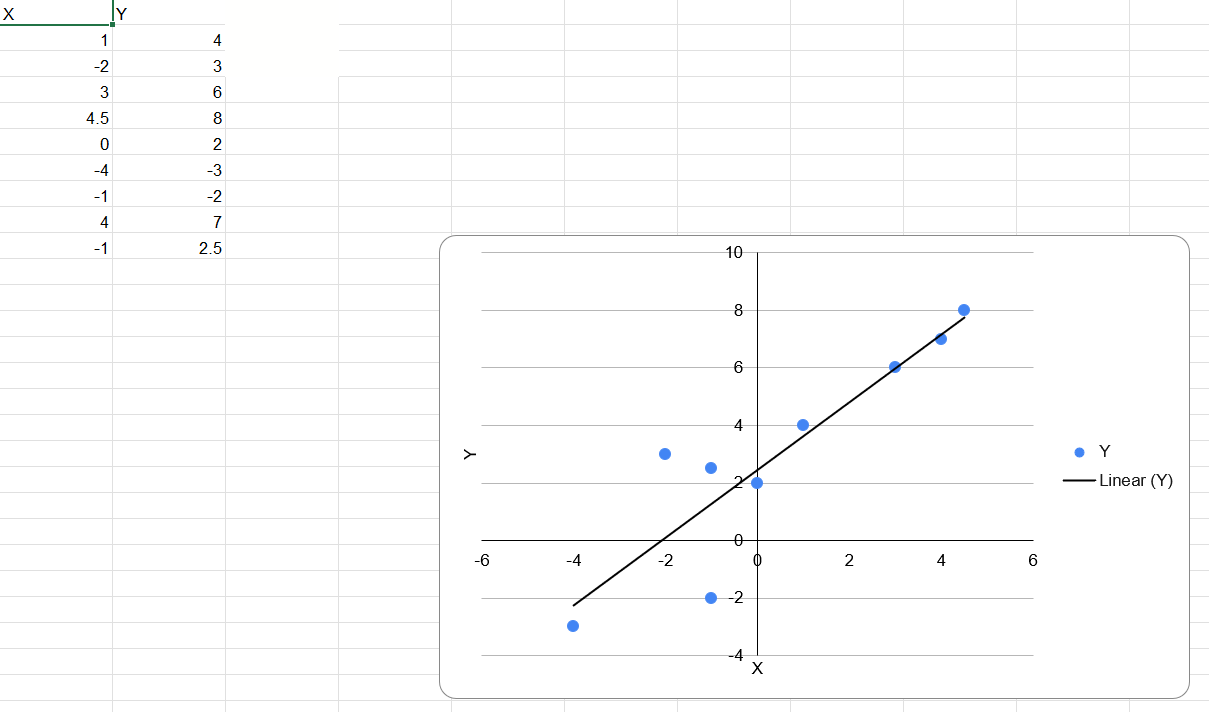
\includegraphics[width=1.0\textwidth]{Module_1_Assignment_Spreadsheet.png}
    \caption{Manual Fitting Excel Chart}
    \label{fig:regression_optimization_excel}
\end{figure}
\begin{figure}[h]
    \centering
    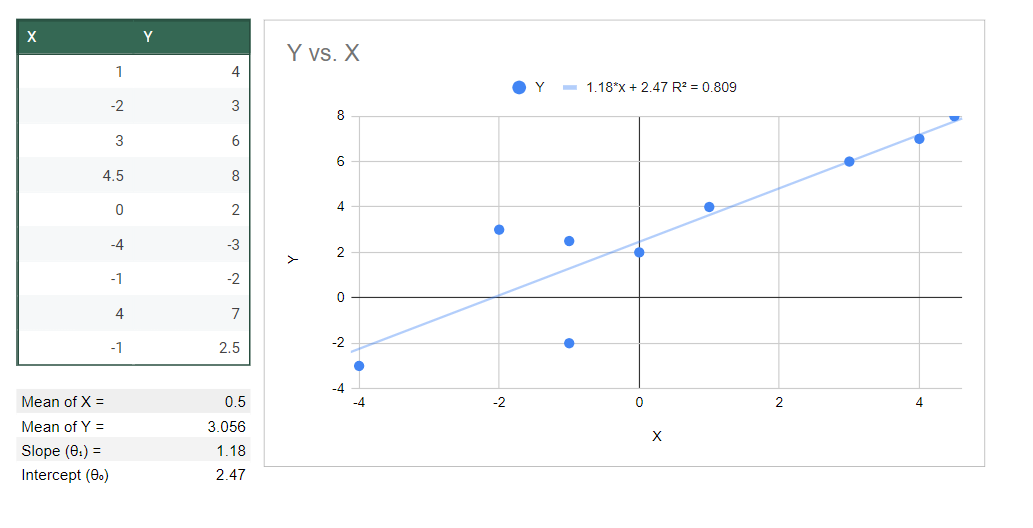
\includegraphics[width=1.0\textwidth]{Regression Model Optimization_ Manual vs Automated.png}
    \caption{Google Sheets' Automatic Fitting Curve}
    \label{fig:work shown}
\end{figure}
\newpage

Your explanation is mostly clear but can be made more precise in terms of how manually fitting vs automatic fitting, and transparency are discussed. Here's an improved version with some added clarity and detail:

In this course, we are provided with an Excel sheet that shows the data points and a trendline, but it does not show the underlying work. Specifically, the Excel chart does not display the equation for the trendline (regression line), making it difficult to know the exact formula used or assess how well the line fits the data. In contrast, the automatic fitting feature in Google Sheets offers more transparency and ease of interpretation. For instance, Google Sheets automatically displays key information such as the equation of the line, slope, intercept, and \(R^2\) value, which quantifies the strength of the relationship between X and Y. \\

In the case of Excel, the \(R^2\) value is not displayed by default, and neither are the equation or parameters of the trendline, unless manually configured. This lack of automatic display reduces transparency, making it harder to evaluate the accuracy or appropriateness of the fit. On the other hand, Google Sheets provides an \(R^2\)
value of 0.809 for this dataset, indicating a strong correlation between X and Y, and it makes these metrics immediately visible, enhancing clarity. \\

Overall, Excel's default trendline visualization lacks transparency compared to Google Sheets, which automatically provides more detailed information, making the relationship between variables easier to interpret.
\end{document}
